\documentclass{beamer}

\usepackage[ngerman]{babel}
\usepackage[T1]{fontenc}
\usepackage{graphicx}
\usepackage{verbatim}
\usepackage{mdwlist}
\usepackage{listings}

\usepackage{xunicode}
\usepackage{xltxtra}
\defaultfontfeatures{Mapping=tex-text}
\setmonofont[Mapping={}, Scale=MatchLowercase]{DejaVu Sans Mono}
\setsansfont[Scale=MatchLowercase]{Linux Biolinum O}
\setmainfont[]{Linux Libertine O}

\newbox\mytempbox
\newdimen\mytempdimen
\newcommand\includegraphicscopyright[3][]{%
  \leavevmode\vbox{\vskip3pt\raggedright\setbox\mytempbox=\hbox{%
  \includegraphics[#1]{#2}}%
    \mytempdimen=\wd\mytempbox\box\mytempbox\par\vskip1pt%
    \fontsize{3}{3.5}\selectfont{\color{black!25}{\vbox{\hsize=\mytempdimen#3}}}\vskip3pt%
}}

\newcommand\prelim[1]{\small }

\newcommand\strColor[1]{\color{beamer@blendedblue}{#1}}

\newcommand\sect[1]{\begin{center}\huge\strColor{#1}\end{center}}

\setbeamerfont{page number in head/foot}{size=\large}
\setbeamertemplate{navigation symbols}{}
\setbeamertemplate{headline}
{%
    \begin{beamercolorbox}{section in head/foot}
        \vskip1em
        \insertsection\hfill
\includegraphics[height=5em]{FULogo_RGB.eps}\hspace{1em}
        \vskip-5.3em
    \end{beamercolorbox}%
}
\setbeamertemplate{footline}[frame number]

\title{OParl-Validator}
\author{Das OParl-Validator-Team}
\institute{Freie Universität Berlin\\Institut für Informatik}
\date{2. Juli 2014}

\begin{document}

\frame{\titlepage}

%\frame{\tableofcontents}

\frame{
    \frametitle{Gliederung}
    \begin{itemize}
        \item Unsere Kunden
        \item Unsere Arbeitsweise
        \item Mockup und erste Diskussionen
        \item Methodologische Anforderungen
        \item Server Anforderungen
        \item Unsere konstruktiven Beiträge zur Spezifikation
        \item Demonstration
    \end{itemize}
}
\frame{
    \frametitle{Unsere Kunden}
        \begin{itemize}
            \item Direkte Kunden
                \begin{itemize}
                    \item Asnprechpartner und treibende Kraft: Marian Steinbach
                    \item Community: Adreas Kuckartz, Stefan
                \end{itemize}
            \item Indirekte Kunden
                \begin{itemize}
                    \item RIS-Hersteller
                        \begin {itemize}
                            \item CC e-Gov GmbH
                            \item PROVOX Systemplanung GmbH
                            \item QuinScape GmbH
                            \item Somacos GmbH und Co. KG
                            \item Sternberg Software-Technik GmbH
                        \end{itemize}
                    \item Zukünftige Projekte, welche mit OParl-konformen Daten leichter realisiert werden können    
                \end{itemize}
            \end{itemize}
        }
\frame {
\frametitle{Unsere Arbeitsweise}
    \begin{itemize}
        \item Regelmäßige Treffen, mit Protokollierung
        \item Regelmäßige Telefonkonferenzen
        \item Verwendung von Trello und GitHub zu realisierung des Kanban Prinzips
        \item Kommuniation mit Hilfe einer Mailingliste
        \item Relativ freie Zusammenarbeit mit unseren direkten Kunden
    \end {itemize}
    
    }

%Ronald Start
\frame{
    
\includegraphics[scale=0.5]{hard_mock_cafe}
}

\frame{
    \frametitle{Hard Mock Café}
    \begin{itemize}
        \item \$ validator --help
        \item CLI Mock
        \item Post an RIS-Hersteller
    \end{itemize}
}

\frame{
    \frametitle{Mock Like an Egyptian}
    \begin{itemize}
        \item Web-Mock für Devs
        \item localhost:5001 -- teste dein System
        \item Kunde: »NOPE«
    \end{itemize}
}

\frame{
    \frametitle{School of Mock}
    \begin{itemize}
        \item Kommando zurück
        \item neues Web-Mock für oparl.org
        \item Validität, Score, Badges
    \end{itemize}
}

\frame{
    \frametitle{Goodies}
    \begin{figure}[h]
        
\includegraphics[scale=0.5]{badge}
        
\includegraphics[scale=0.4]{score_button}
    \end{figure}
}

\frame{
    \frametitle{Architektur}
    \begin{figure}[h]
        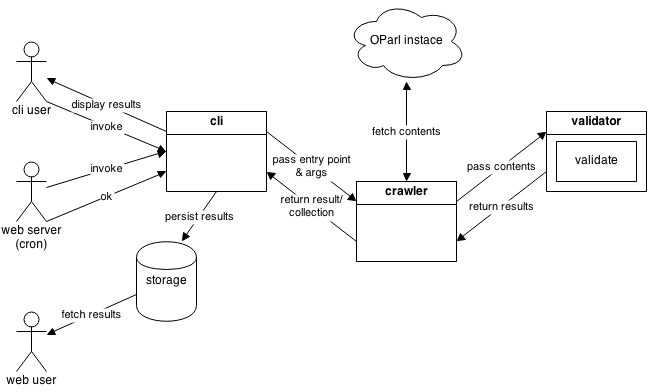
\includegraphics[scale=0.4]{architecture}
    \end{figure}
}
%Ronald Ende

\frame{
    \frametitle{Methodologische Anforderungen}
    \begin{itemize}
        \item JSON Schema
        \item PEP 8
        \item Coverage
        \item Travis CI
        \item OParl PyPI account
    \end{itemize}
}

\begin{frame}[fragile]
    \frametitle{Server-Anforderungen}
    \begin{itemize}
        \item Liste der Anforderungen
        \item JSON Schema
        \item Proprietäre Erweiterungen
            \begin{lstlisting}[basicstyle=\footnotesize\tt, xleftmargin=-64pt]
                "oparl:validate": [
                    {
                        "message": "name and nameShort must not be equal",
                        "section": "5.2.3",
                        "method": "oparlvalidator.schema:name_not_equal_shortName"
                    }
                ]
            \end{lstlisting}
    \end{itemize}
\end{frame}

\frame{
    \frametitle{Unsere Beiträge zur Spezifikation}
    \begin{itemize}
        \item Häufige Änderungen an der Spezifikation trotz Reviewphase
        \item Kleine Änderungen: vier Pull Requests, vier Issues
        \item Feedback zur Verwendung von JSON-LD gegeben
    \end{itemize}
}

\begin{frame}[fragile]
    \frametitle{JSON-LD}

    \begin{lstlisting}[basicstyle=\footnotesize\tt, xleftmargin=-32pt]
        {
            "@context": [
                {
                    "oparl": "http://oparl.org/specs/1.0/schema/",
                    "rdfs": "http://www.w3.org/TR/rdf-schema/#",
                    "body": {
                      "@id": "oparl:body",
                      "@type": "@id"
                    },
                    "name": "rdfs:label"
                }
            ],
            "@type": "oparl:Meeting",
            "body": "http://ris.exmaple.org/body/0",
            "name": "Erste Sitzung"
        }
    \end{lstlisting}
\end{frame}

\begin{frame}[fragile]
    \frametitle{JSON-LD}
    \begin{lstlisting}[basicstyle=\footnotesize\tt, xleftmargin=-32pt]
        [
            {
                "@type": [
                    "http://oparl.org/specs/1.0/schema/Meeting"
                ],
                "http://oparl.org/specs/1.0/schema/body": [
                    {
                        "@id": "http://ris.exmaple.org/body/0"
                    }
                ],
                "http://www.w3.org/TR/rdf-schema/#label": [
                    {
                        "@value": "Erste Sitzung"
                    }
                ]
            }
        ]
    \end{lstlisting}
\end{frame}

\end{document}
